\documentclass[11pt]{article}
\pdftrailerid{}
\usepackage[T1]{fontenc}
\usepackage{lmodern}
\usepackage[margin=1in]{geometry}
\usepackage{amsmath,amssymb,amsthm,mathtools}
\usepackage{mathrsfs}
\usepackage{microtype}
\usepackage{enumitem}
\usepackage{booktabs}
\usepackage{tikz}
\usetikzlibrary{arrows.meta,positioning}
\usepackage[colorlinks=true,linkcolor=blue!45!black,citecolor=blue!45!black,urlcolor=blue!45!black]{hyperref}
\hypersetup{pdftitle={Hardness of finding large independent sets in three-colorable graphs},pdfauthor={OpenAI}}
\newtheorem{theorem}{Theorem}[section]
\newtheorem{lemma}[theorem]{Lemma}
\newtheorem{proposition}[theorem]{Proposition}
\newtheorem{corollary}[theorem]{Corollary}
\theoremstyle{definition}
\newtheorem{definition}[theorem]{Definition}
\theoremstyle{remark}
\newtheorem{remark}[theorem]{Remark}
\newcommand{\T}{\mathbb T}
\newcommand{\R}{\mathbb R}
\newcommand{\Q}{\mathbb Q}
\newcommand{\N}{\mathbb N}
\newcommand{\E}{\mathbb E}
\newcommand{\eps}{\varepsilon}
\DeclareMathOperator{\dist}{dist}
\DeclareMathOperator{\Lip}{Lip}
\DeclareMathOperator{\val}{val}
\DeclareMathOperator{\id}{id}
\setlist{itemsep=3pt,topsep=5pt}
\setlength{\emergencystretch}{2em}
\title{Hardness of finding large independent sets\\in three-colorable graphs}
\author{OpenAI}
\date{September 24, 2026}
\begin{document}
\maketitle
\begin{abstract}
We prove that, for every fixed $0<\delta<1/3$, it is NP-hard to distinguish
three-colorable graphs from graphs in which every independent set has fewer
than $\delta$ times the number of vertices. Consequently, for every fixed
integer $c\ge3$, finding a proper $c$-coloring of a three-colorable graph is
NP-hard.
\end{abstract}
\section{Introduction}

A proper coloring of a graph assigns different colors to adjacent vertices.
An independent set is a set of pairwise nonadjacent vertices.
For a nonempty finite graph $G$, write $n=|V(G)|$ and let $\alpha(G)$
be its maximum independent-set size.
Every three-colorable graph contains an independent set of size at least
$n/3$: one of its three color classes has that size.
We prove that distinguishing this structured case from graphs with an
arbitrarily small fixed independence ratio is NP-hard.

\begin{theorem}\label{thm:main}
For every fixed real $0<\delta<1/3$, there is a deterministic
polynomial-time algorithm $R_\delta$ that maps each explicitly encoded
Boolean $3$-CNF formula $\phi$ to a nonempty finite simple undirected
unweighted graph $G_\phi$ such that
\[
 \begin{array}{ll}
 \phi\text{ is satisfiable}
   &\Longrightarrow G_\phi\text{ is three-colorable},\\[2pt]
 \phi\text{ is unsatisfiable}
   &\Longrightarrow \alpha(G_\phi)<\delta\,|V(G_\phi)|.
 \end{array}
\]
The running time and explicit output size are polynomial in the ordinary
binary encoding length of $\phi$. Their constants and polynomial degree
may depend on the fixed $\delta$, but not on $\phi$.
The coloring in the first implication covers every vertex and is not
supplied with the graph.
\end{theorem}

It suffices to prove Theorem~\ref{thm:main} for rational $\delta$.
For a fixed real threshold, choose a fixed rational $0<\delta_0<\delta$
and use $R_{\delta_0}$. We assume $\delta$ rational in the construction
and its analysis.
The density conclusion is stronger than an arbitrarily large fixed
lower bound on chromatic number. Indeed, small independence ratio forces
large chromatic number, whereas adjoining isolated vertices preserves
chromatic number and can make the independence ratio arbitrarily close
to one.

Approximate graph coloring asks, for fixed integers $3\le k\le c$,
to find a proper $c$-coloring of a graph promised to be $k$-colorable.
Its decision version distinguishes $k$-colorable graphs from graphs
that are not $c$-colorable. The following consequence recovers the
constant-palette hardness theorem.

\begin{corollary}\label{cor:coloring}
For every fixed pair of integers $3\le k\le c$, it is NP-hard to
distinguish $k$-colorable graphs from graphs that are not $c$-colorable.
\end{corollary}

\begin{proof}
Choose a rational $0<\delta<\min\{1/3,1/c\}$ and apply
Theorem~\ref{thm:main}. A three-colorable graph is $k$-colorable.
A $c$-colorable graph has an independent set of size at least $n/c$,
which the soundness bound excludes.
\end{proof}

\subsection{History and comparison with prior work}

The difficulty of approximate coloring persists even with a very small
promised palette. Khanna, Linial, and Safra established hardness of
four-coloring three-colorable graphs \cite{KhannaLinialSafra2000};
Guruswami and Khanna later gave a different proof and obtained
bounded-degree and edge-error variants \cite{GuruswamiKhanna2004}.
The algebraic theory of promise constraint satisfaction developed by
Barto, Bul\'{\i}n, Krokhin, and Opr\v{s}al gave hardness of
$(2k-1)$-coloring $k$-colorable graphs, and hence five colors when
$k=3$ \cite[Theorem~6.5]{BartoBulinKrokhinOprsal2021}.
Their Example~2.9 records the conjectured hardness for every fixed
$3\le k\le c$.

Guruswami and Sandeep showed that the ordinary $d$-to-$1$ Games
Conjecture with perfect completeness, for any fixed $d\ge2$, implies
constant-palette hardness for three-colorable graphs
\cite[Theorem~1]{GuruswamiSandeep2020}.
Their reduction first gives arbitrarily small independent-set density
with a $2d$-colorable completeness promise
\cite[Theorem~9]{GuruswamiSandeep2020}. The arc-graph reduction of
Krokhin, Opr\v{s}al, Wrochna, and \v{Z}ivn\'y
\cite[Theorem~1.8]{KrokhinOprsalWrochnaZivny2023} then reduces the
promised palette to three for the coloring conclusion. The resulting
three-colorable hardness statement does not include the independent-set
guarantee.
The companion article~\cite[Theorem~1.1]{OpenAIPerfectCompleteness2026}
establishes the ordinary perfect-completeness premise for $d=2$.

Fei, Minzer, and Wang have proved the $4$-to-$1$ Games Conjecture
with perfect completeness \cite[Theorem~1.6]{FeiMinzerWang2026}.
Combining it with the preceding reductions resolves the constant-palette
conjecture: their Corollary~1.7 gives the three-colorable versus not
$c$-colorable gap for every fixed $c$. Their Corollary~1.9 gives
arbitrarily small independent-set density with an eight-colorable
completeness promise, corresponding to $2d=8$.
Theorem~\ref{thm:main} combines this stronger form of soundness with
three-colorability of the entire graph. Our proof starts with ordinary
projection Label Cover and does not require a bound on projection-fiber
sizes.

The distinction between colorability and independence density also
appears in earlier conditional results. Dinur, Mossel, and Regev obtained
three-colorable completeness and arbitrarily small independent-set
soundness from their fish-shaped Label Cover conjecture
\cite[Conjecture~4.8 and Sections~4.3--4.5]{DinurMosselRegev2009}.
Braverman, Khot, Lifshitz, and Minzer obtained the same graph promise
from the Rich $2$-to-$1$ Games Conjecture using their invariance principle
for the multi-slice \cite[Corollary~1.19]{BravermanKhotLifshitzMinzer2022}.
The Rich condition requires that, at each left question, a uniformly
random incident constraint induce a uniformly random partition of the
left alphabet among all partitions into pairs. This is not part of the
ordinary $2$-to-$1$ premise above.

A different line of work relaxes completeness by permitting deletion
of a small fraction of vertices. Dinur, Khot, Perkins, and Safra proved
that, for arbitrarily small fixed $\varepsilon>0$, it is NP-hard to find
an independent set of density $1/9$ when an induced
three-colorable subgraph occupies at least $(1-\varepsilon)n$ vertices
\cite{DinurKhotPerkinsSafra2010}.
Hecht, Minzer, and Safra subsequently proved, under randomized reductions,
hardness of almost coloring such almost-three-colorable graphs with any
fixed palette \cite{HechtMinzerSafra2023}.
The all-vertex completeness in Theorem~\ref{thm:main} retains the original
coloring promise, while allowing every fixed positive soundness density.

Algorithmic work gives a complementary perspective on the remaining
quantitative gap. Bansal, Huang, and Lee give a polynomial-time algorithm
using $O(n^{0.19539})$ colors \cite{BansalHuangLee2026}, improving the
$\widetilde O(n^{0.19747})$ bound of Kawarabayashi, Thorup, and Yoneda
\cite{KawarabayashiThorupYoneda2024}.
In preprints posted after the September 24 version of this manuscript,
Narang and Tang report a randomized polynomial-time bound of
$O(n^{(13-\sqrt{97})/18+\varepsilon})$ for each fixed
$\varepsilon>0$ \cite{NarangTang2026}, and Anand reports a randomized
polynomial-time bound of $O(n^{4/23})$ \cite{Anand2026}.
Our reduction has fixed $\delta$ and fixed palettes; its polynomial
exponent can depend on these constants.

\subsection{Proof overview and method ancestry}

The starting problem is Label Cover: a bipartite collection of questions
and tests, each prescribing a projection from a left answer to a right
answer. The PCP theorem and parallel repetition supply instances in
which either every test can be satisfied or every labeling succeeds
on at most an arbitrarily small fixed fraction of tests
\cite{AroraEtAl1998,Raz1998,DinurSteurer2014}.

We replace one left question at a time by a right question, obtaining
chains of question tuples. This use of layered tuples and projection
constraints is related to the multilayered PCP construction of
Dinur, Guruswami, Khot, and Regev \cite{DinurGuruswamiKhotRegev2005}.
At each tuple, a point assigns a phase in $\T=\R/\mathbb Z$ to every
possible product answer. An answer projection $\pi:M\to M' $ pulls a
phase vector $x\in\T^{M'}$ back to $x\circ\pi\in\T^M$.
Link these two points with length zero, and link points within each
phase space with their sup circle distance. Shortest paths through
these links define a pseudometric. Edges compare one point with
the coordinatewise half-shift of another. A satisfying Label Cover
labeling evaluates each phase assignment at one product answer.
This evaluation is nonexpanding, and the edge threshold forces adjacent
vertices to have circle phases more than $1/3$ apart. Three equal
half-open intervals of the circle therefore color all vertices properly.

For soundness, an independent set gives bounded functions on the tuple
phase spaces that change sign under a half-shift and satisfy a common
Lipschitz bound. Austin's dimension-independent approximation theorem
\cite{Austin2016}, a continuous counterpart of Friedgut's junta theorem
\cite{Friedgut1998}, approximates these functions using boundedly many
answer coordinates. The difficulty is that approximation under product
measure need not survive identifications of coordinates by projections.
We therefore choose coordinate lists for whole small subchains and
introduce independent rotation variables at every layer of each
subchain. All required compatibility properties are proved within this
paper. Projecting the selected coordinates to the last layer places
all lists in a common answer set. A shared answer for two separated
subchains supplies compatible answers to an intervening Label Cover
test, so low source value makes these intersections rare.

Two further steps turn this structural information into a density
bound. First, a distributional alignment lemma chooses a law on sets
of layers before seeing the lists. On most selected sets, each listed
label can be assigned to an index shared by all its occurrences.
The bound is independent of the label universe. The proof combines
finite minimax, Ramsey homogenization of finite probability patterns,
and an order-invariant random-array argument. The homogenization step
has antecedents in the Ramsey theory of random variables
\cite{TrotterWinkler1998}; we give the particular alignment argument
in full.

Second, we sample coefficients at finitely many levels between $0$ and
$1$, with geometrically decreasing probabilities. Enough layers make
a coefficient equal to $1$ likely. That layer absorbs auxiliary uniform
phase shifts without changing their distribution. Alignment makes
dependence on a zero-coefficient layer small; decreasing a positive
coefficient by one level bounds its probability of substantial
dependence. A dimension-independent bound on influential coordinates
then gives a small mean square, and hence a small independent-set density.

Only fixed finite rational data enter the graph construction.
The probability experiment is expanded exactly into unweighted vertices,
so the reduction is deterministic.
Section~\ref{sec:preliminaries} states the standard inputs and derives
the analytic coordinate bounds.
Section~\ref{sec:construction} constructs the graph with finite parameters
and proves completeness. Section~\ref{sec:lists} extracts the coordinate
lists from an independent set and decodes intersections of separated lists.
Section~\ref{sec:alignment} states distributional alignment and applies
it to these lists. Section~\ref{sec:coefficient} proves the coefficient
estimate under explicit inequalities, and Section~\ref{sec:parameters}
chooses all constants in dependency order and completes
Theorem~\ref{thm:main}. The self-contained proof of distributional
alignment is given in Section~\ref{sec:alignment-proof}.

\section{Two standard inputs and an analytic consequence}
\label{sec:preliminaries}

We first state the two established results used in the reduction.
The new combinatorial and analytic arguments will be proved in full.
For a positive integer $r$, write $[r]=\{1,\ldots,r\}$.
All products of metric spaces carry the sup metric unless stated otherwise.
The circle $\T=\R/\mathbb Z$ carries the distance
$d_{\T}(x,y)=\min_{k\in\mathbb Z}|x-y-k|$.
Uniform inputs on a cube have product Lebesgue law, and uniform inputs on
a product of circles have product Haar law. Norms $\|\cdot\|_p$
always use the indicated probability measure.
An empty sum is zero.

\subsection{A projection constraint problem}

A \emph{Label Cover instance} consists of finite question sets $U,V$,
nonempty finite answer alphabets $\Sigma_L,\Sigma_R$, and a nonempty
explicit list $\mathcal C$ of test occurrences.
An occurrence $c$ has questions $u_c\in U$, $v_c\in V$, and a total map
$\pi_c:\Sigma_L\to\Sigma_R$.
The value is
\[
 \val(\mathcal C)=
 \max_{\ell:U\to\Sigma_L,\ \rho:V\to\Sigma_R}
 \Pr_{c\in\mathcal C}\bigl[\pi_c(\ell(u_c))=\rho(v_c)\bigr],
\]
where occurrences, including repeated occurrences, are sampled uniformly.

\begin{theorem}[Perfect-completeness Label Cover]\label{thm:label-cover}
For every fixed rational $\sigma\in(0,1)$ there are nonempty constant
alphabets and a deterministic polynomial-time reduction from $3$SAT to
explicit Label Cover instances with nonempty occurrence lists such that
satisfiable formulas have value $1$ and unsatisfiable formulas have value
at most $\sigma$.
\end{theorem}

This is the standard consequence of the PCP Theorem and parallel
repetition \cite{AroraEtAl1998,Raz1998}. A quantitative statement is
\cite[Theorem~6.2, full version]{DinurSteurer2014}:
for a fixed number $k$ of repetitions, the output size is $n^{O(k)}$,
the alphabet size is at most $a^k$, and the soundness is at most $\beta_0^k$,
for absolute constants $a>1$ and $0<\beta_0<1$.
Choose a fixed $k$ for which $\beta_0^k\le\sigma$.
The unweighted total-projection formulation is explicitly recorded in
\cite[Definitions~1.1--1.2 and Theorem~1.3]{DKKMS2025}.
The latter source even supplies $d$-to-one maps, a property we do not use.
Here the verifier's random choices specify an explicit list of constraints;
they are not random choices of the reduction.
Unused questions can be removed.

\subsection{Juntas for the sup metric}

A function is a \emph{junta on $S$} if it depends only on the input
coordinates in $S$. The approximating functions below need not be continuous.
We use Austin's continuous junta theorem \cite{Austin2016}, which
extends the dimension-independent coordinate approximation phenomenon
of Friedgut's Boolean junta theorem \cite{Friedgut1998}.

\begin{theorem}[Dimension-independent junta approximation]
\label{thm:junta}
For every $0\le L<\infty$ and $\tau>0$ there is an integer $J(L,\tau)\ge1$
such that every $L$-Lipschitz function
$f:[0,1]^N\to[-1,1]$, for every positive integer $N$, admits a junta
on at most $J(L,\tau)$ coordinates with $L^2$ error less than $\tau$.
The junta may be taken to be a coordinate conditional expectation of $f$.
\end{theorem}

To obtain this formulation from
\cite[Theorem~1.1, arXiv version~4]{Austin2016},
use the usual interval with uniform measure and modulus of continuity
$\omega(t)=Lt$. The interval is compact, connected, and locally connected,
as required there. Austin's theorem gives
$\|f-\E[f\mid X_S]\|_1<\tau^2/2$ with $|S|$ bounded independently of $N$.
Both functions take values in $[-1,1]$, so
\[
 \|f-\E[f\mid X_S]\|_2^2
 \le 2\|f-\E[f\mid X_S]\|_1<\tau^2.
\]
The bound applies to pullbacks of torus functions, since the quotient
$[0,1]^N\to\T^N$ is nonexpanding and preserves the product uniform law.

For a square-integrable function $H$ of independent circle coordinates
$z_1,\ldots,z_s$, let $E_i$ average coordinate $z_i$ alone, and set
\[
 Q_i=\id-E_i,\qquad D_i(H)=\|Q_iH\|_2.
\]
Both $E_i$ and $Q_i$ are orthogonal projections. In particular,
$\|Q_if\|_2\le\|f\|_2$; the constant here is one.

\begin{lemma}[Two dimension-independent bounds]\label{lem:influences}
Fix $0\le L<\infty$ and $\eps>0$. There are $\beta>0$ and an integer $K\ge1$,
independent of $s$, such that every $L$-Lipschitz
$H:\T^s\to[-1,1]$ satisfies:
\begin{enumerate}[label=\textup{(\roman*)}]
\item if $\E H=0$ and $\E H^2>\eps$, then $D_i(H)\ge\beta$ for some $i$;
\item at most $K$ indices satisfy $D_i(H)\ge\beta/2$.
\end{enumerate}
\end{lemma}

\begin{proof}
Let $J=J(L,\sqrt{\eps}/2)$ from Theorem~\ref{thm:junta}.
Choose a set $S$ of at most $J$ coordinates such that
$G=\E[H\mid z_S]$ satisfies $\|H-G\|_2<\sqrt{\eps}/2$.
If $H$ has mean zero and squared norm exceeding $\eps$, then
$G$ has mean zero and, by orthogonality,
$\|G\|_2^2>3\eps/4$, in particular $\|G\|_2^2>\eps/4$.

For completeness, decompose
\[
 H=\sum_{A\subseteq[s]} H_A,\qquad
 H_A=\Bigl(\prod_{i\in A}Q_i\Bigr)
     \Bigl(\prod_{i\notin A}E_i\Bigr)H .
\]
The factors commute and the summands are orthogonal.
Thus $G=\sum_{A\subseteq S}H_A$ and, in the mean-zero case,
\[
 \|G\|_2^2
 =\sum_{\varnothing\ne A\subseteq S}\|H_A\|_2^2
 \le \sum_{i\in S}\sum_{A\ni i}\|H_A\|_2^2
 =\sum_{i\in S}D_i(H)^2.
\]
Consequently $\beta=\sqrt{\eps/(4J)}$ works in (i).

For (ii), use Theorem~\ref{thm:junta} again with error less than
$\beta/2$, and write $G'$ for the resulting junta, on at most
$K=J(L,\beta/2)$ coordinates. If $i$ is not one of these coordinates,
then $Q_iG'=0$, so
\[
 D_i(H)=\|Q_i(H-G')\|_2\le\|H-G'\|_2<\beta/2.
\]
This proves the cardinality bound.
\end{proof}

The first part locates a coordinate when the function has substantial
variance; the second limits how many coordinates can have a smaller
but still fixed amount of dependence. Their simultaneous dimension
independence is what will permit the number of test blocks to be chosen
after both bounds are fixed.

\section{The finite graph reduction}
\label{sec:construction}

We first construct a graph from an arbitrary Label Cover instance and
fixed finite parameters. A satisfying labeling will give its
three-coloring. The following sections analyze independent sets and
determine which parameter choices make their density small.

Fix integers $r\ge s\ge2$ and $m\ge1$, an even positive integer $P$,
a rational $\lambda\in(0,1)$, and a rational probability distribution
$\mu$ on $\binom{[r]}s$. Set $D=mP$. The coefficient values and their
probabilities are
\begin{equation}\label{eq:coefficient-law}
 \mathcal T_m=\{0,1/m,\ldots,1\},\qquad
 p_k=\Pr(t=k/m)=\frac{\lambda^k}{\sum_{\ell=0}^m\lambda^\ell}
 \quad(0\le k\le m).
\end{equation}
These finite data are inputs to the construction. Section~\ref{sec:parameters}
will choose them as constants depending only on the target density
$\delta$, before choosing the Label Cover soundness and alphabets.
The finite probability experiment below specifies a deterministic list
of vertices by expanding each rational probability into a multiplicity.

Choose a fixed integer $q>1/\delta$. Before invoking Label Cover,
reindex the occurring variables densely, preserving repeated occurrences
of each variable. Remove tautological clauses and duplicate literals.
A formula with no clauses maps directly to a one-vertex graph; a formula
containing an empty clause maps directly to $K_q$.
Pad a remaining short clause to width three by including all sign choices
for fresh filler variables. This preserves satisfiability at constant
overhead. In the remainder, the formula has only nonempty clauses and
has passed through this preprocessing.

\subsection{Tuples, grids, and zero-length links}

Let $\mathcal C$ be any Label Cover instance, with unused questions
removed. In layer $i\in[r]$, take all question
tuples
\[
 \mathbf q=(v_1,\ldots,v_{i-1},u_i,\ldots,u_{r-1})
 \in V^{i-1}\times U^{r-i}.
\]
The answer set of such a tuple is
\[
 M_i=\Sigma_R^{\,i-1}\times\Sigma_L^{\,r-i}.
\]
Layered products of questions with projection constraints also occur in
the multilayered PCP construction of \cite{DinurGuruswamiKhotRegev2005}.
Here each position is a separate coordinate even if question names repeat.
Different tuples in a layer use separate copies of this same answer set.

Between adjacent layers $i$ and $i+1$, impose a map whenever the
tuples agree outside position $i$ and their questions at position $i$
are the endpoints of a test occurrence $c$.
The map on answer sets applies $\pi_c$ in position $i$ and the identity
in every other position. Impose it separately for every occurrence.

Write $\Gamma=(D^{-1}\mathbb Z)/\mathbb Z$.
At each question tuple place a separate copy of $\Gamma^{M_i}$,
and let $\mathscr X$ be their disjoint union.
Make a finite undirected weighted link graph on $\mathscr X$:
\begin{itemize}
\item Within each copy, link any two points with length their sup circle
distance.
\item For every imposed map $\pi:M_i\to M_{i+1}$, link each target
point $x\in\Gamma^{M_{i+1}}$ to its source pullback $x\circ\pi$
with length zero.
\end{itemize}
Let $\dist$ be the resulting shortest-path extended pseudometric,
with distance infinity between components.
Thus distinct points may have distance zero.

Let $T$ add $1/2$ to every phase coordinate, within each copy.
Since $D$ is even, $T$ permutes $\mathscr X$ and satisfies $T^2=\id$.
It preserves all link lengths and therefore is an isometry of $\dist$.

If some $x\in\mathscr X$ satisfies
\begin{equation}\label{eq:clique-test}
 \dist(x,Tx)\le1/8,
\end{equation}
output $K_q$ and stop. This branch already has independent-set density
$1/q<\delta$. We will show that it never occurs in completeness.

\subsection{Vertices and edges}

If \eqref{eq:clique-test} fails for every point, consider the following
finite experiment.

\begin{enumerate}
\item Sample $r-1$ independent uniform occurrences
$c_1,\ldots,c_{r-1}$, with questions $(u_h,v_h)$ at position $h$.
They determine a chain of tuples
\[
 \mathbf q_i=(v_1,\ldots,v_{i-1},u_i,\ldots,u_{r-1}),
 \qquad i\in[r].
\]
Write $\pi_{ij}:M_i\to M_j$ for the corresponding composite answer maps.
They apply the test projections in positions $i,\ldots,j-1$
and leave the other positions unchanged; in particular they are
composition-consistent.

\item Independently choose $B\sim\mu$.
For every $j\in B$, independently choose $t_j$ from
\eqref{eq:coefficient-law}, and choose independent rotation entries
\[
 \widehat\theta_{j,\ell}\ \text{uniform in }\
 \{0,1/P,\ldots,(P-1)/P\},\qquad \ell\in M_j .
\]

\item With $b=\min B$, give the outcome the location
\begin{equation}\label{eq:location}
 x=\left(
 \sum_{j\in B}t_j\widehat\theta_{j,\pi_{bj}(\kappa)}
        \pmod1\right)_{\kappa\in M_b}
 \in\Gamma^{M_b}
\end{equation}
in the copy at tuple $\mathbf q_b$.
\end{enumerate}

Take distinct output vertices for these elementary outcomes with
integer multiplicities that make the experiment their exact uniform law.
The existence and size of these multiplicities are verified below.
Different vertices may have the same location.
For distinct vertices with locations $x,y$, put an edge precisely when
\begin{equation}\label{eq:edge}
 \dist(x,Ty)\le1/8.
\end{equation}
This is symmetric because $T$ is an involutive isometry:
$\dist(x,Ty)=\dist(Tx,y)=\dist(y,Tx)$.

\begin{proposition}[Explicit deterministic encoding]\label{prop:encoding}
For fixed choices of the parameters and Label Cover alphabets, this rule
constructs a nonempty finite simple
unweighted graph in deterministic polynomial time and output size,
measured in the size of the explicit Label Cover instance. Composing
with Theorem~\ref{thm:label-cover} for any fixed $\sigma$ gives polynomial
time and output size in the binary encoding length of the original
$3$-CNF formula.
\end{proposition}

\begin{proof}
Let $N=|\mathcal C|\ge1$.
All alphabets, layer counts, and grids are fixed constants.
There are polynomially many question tuples, each with a constant-size
grid. The imposed maps and links are therefore polynomially enumerable.
Every finite link length is an integer multiple of $1/D$.
After multiplying lengths by $D$, exact integer shortest-path algorithms
compute all distances, with infinity stored separately.
Shortest paths have polynomial bit length, and comparison with $1/8$
is exact by multiplication by $8$. This also implements the clique test.

There are exactly $N^{r-1}$ equally likely occurrence chains.
For each chain, the remaining outcome probabilities are fixed rational
numbers. The number of rotation entries can vary with $B$ and its layers,
but it ranges over fixed constants. Choose a common positive denominator
$C_0$ for all these conditional probabilities. For a conditional outcome
of probability $p$, emit $C_0p$ distinct vertices, omitting zero-probability
outcomes. Every chain then contributes exactly $C_0$ vertices.
The total is $C_0N^{r-1}$, and uniform sampling of these vertices is
exactly the stated experiment, followed by a uniform choice among the
copies of the chosen outcome. Exhaustive enumeration uses no random
bits. Evaluating \eqref{eq:edge} for every distinct pair remains
polynomial and gives an explicit edge list with no loops or multiple edges.

The Label Cover reduction is polynomial for the fixed $\sigma$.
The initial variable reindexing and clause preprocessing take polynomial
time in the ordinary binary input length; the two trivial branches have
constant-size outputs. Thus the construction covers every explicitly
encoded $3$-CNF formula.
\end{proof}

\begin{lemma}[All-vertex completeness]\label{lem:completeness}
If the Label Cover instance has value $1$, the clique branch does not
occur and the constructed graph has a proper three-coloring.
\end{lemma}

\begin{proof}
Fix a labeling satisfying every occurrence. At each question tuple,
form the product of its assigned answers, an element of that tuple's
answer set. Evaluate a grid point at this product answer.
This defines a map $\varphi:\mathscr X\to\T$.

Within a copy, evaluation is nonexpanding for the sup circle distance.
Across each zero link the two evaluations agree because the labeling
satisfies that test occurrence. Hence $\varphi$ is nonexpanding for
every path, and thus for $\dist$.
Also $\varphi(Tx)=\varphi(x)+1/2$.
Consequently $\dist(x,Tx)\ge1/2$ for every $x$, so the clique test fails.

If output vertices at $x,y$ are adjacent, then
\[
 d_{\T}\bigl(\varphi(x),\varphi(y)+1/2\bigr)\le1/8,
 \qquad
 d_{\T}\bigl(\varphi(x),\varphi(y)\bigr)\ge3/8>1/3.
\]
Color each vertex according to which of the half-open intervals
$[0,1/3)$, $[1/3,2/3)$, $[2/3,1)$ contains its phase.
Two phases in the same interval have circle distance less than $1/3$,
so this colors every vertex properly. All multiplicity copies receive
the color of their location.
\end{proof}

Figure~\ref{fig:geometry} shows how the two parts of the construction
serve this coloring: projection links preserve the evaluated phase,
whereas an output edge separates its endpoint phases by more than the
length of a color interval.

\begin{figure}[t]
\centering
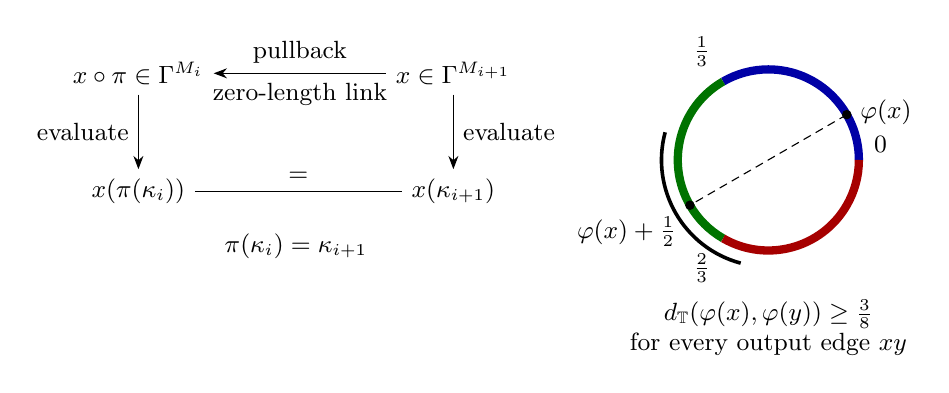
\begin{tikzpicture}[>=Stealth,every node/.style={font=\small}]
\node (source) at (0,1.1) {$x\circ\pi\in\Gamma^{M_i}$};
\node (target) at (4.0,1.1) {$x\in\Gamma^{M_{i+1}}$};
\draw[<-] (source) -- node[above] {pullback} node[below] {zero-length link} (target);
\node (seval) at (0,-0.4) {$x(\pi(\kappa_i))$};
\node (teval) at (4.0,-0.4) {$x(\kappa_{i+1})$};
\draw[->] (source) -- node[left] {evaluate} (seval);
\draw[->] (target) -- node[right] {evaluate} (teval);
\draw (seval) -- node[above] {$=$} (teval);
\node at (2.0,-1.1) {$\pi(\kappa_i)=\kappa_{i+1}$};
\begin{scope}[shift={(8.0,0)},scale=1.15]
\draw[line width=3pt,blue!65!black] (1,0) arc[start angle=0,end angle=120,radius=1];
\draw[line width=3pt,green!45!black] (120:1) arc[start angle=120,end angle=240,radius=1];
\draw[line width=3pt,red!65!black] (240:1) arc[start angle=240,end angle=360,radius=1];
\draw[densely dashed] (30:1) -- (210:1);
\fill (30:1) circle[radius=1.5pt];
\fill (210:1) circle[radius=1.5pt];
\node[right] at (30:1.05) {$\varphi(x)$};
\node[below left] at (210:1.05) {$\varphi(x)+\tfrac12$};
\draw[line width=1.3pt] (165:1.18) arc[start angle=165,end angle=255,radius=1.18];
\node at (8:1.25) {$0$};
\node[above left] at (120:1.07) {$\tfrac13$};
\node[below left] at (240:1.07) {$\tfrac23$};
\node[align=center] at (0,-1.85) {$d_{\T}(\varphi(x),\varphi(y))\ge\tfrac38$\\for every output edge $xy$};
\end{scope}
\end{tikzpicture}
\caption{The auxiliary geometry and the output coloring. Left: a satisfying
product answer makes evaluation agree across a projection link. Here
$\kappa_i$ and $\kappa_{i+1}$ are the satisfying product answers at the
two tuples. The answer
map $\pi:M_i\to M_{i+1}$ and its phase pullback go in opposite directions.
Right: the three arcs represent the half-open color intervals. For the
illustrated phase $\varphi(x)$, the black outer arc contains the possible
phases $\varphi(y)$ of its neighbors, within $1/8$ of the antipodal phase.
The weighted links on the left define the pseudometric; the output graph
uses the separate half-shift edge rule.}
\label{fig:geometry}
\end{figure}

\section{From an independent set to bounded subchain lists}
\label{sec:lists}

Fix $\sigma\in(0,1)$ and assume that the Label Cover value is at most $\sigma$.
The clique branch already has the required soundness, so suppose
it does not occur. Fix a nonempty independent vertex set $\mathcal A$
in the output graph. We first turn it into functions on the tuple tori,
then approximate their restrictions to small subchains using bounded
coordinate lists. Source soundness will show that lists belonging to
separated subchains are usually disjoint. Throughout the analysis, set
$L=64$.

\subsection{Odd functions and compatibility}

Let $A\subseteq\mathscr X$ be the set of locations of vertices in
$\mathcal A$, with multiplicities removed. Then
\begin{equation}\label{eq:independent-separation}
 \dist(A,TA)>1/8.
\end{equation}
For locations of distinct selected vertices this follows from the missing
edge in \eqref{eq:edge}. For a point compared with itself, it follows
from exclusion of \eqref{eq:clique-test}. Since the sets are finite,
these pointwise strict inequalities give \eqref{eq:independent-separation},
including when distances are infinite.

On $\mathscr X$ define
\begin{equation}\label{eq:bumps}
 f(x)=\bigl(1-32\dist(x,A)\bigr)_+
       -\bigl(1-32\dist(Tx,A)\bigr)_+,
 \qquad (u)_+=\max\{u,0\},
\end{equation}
with each bump defined to be zero at infinite distance.
This function takes values in $[-1,1]$, satisfies $f(Tx)=-f(x)$,
and equals $1$ on $A$.
It is constant across every zero link.
Within each grid copy it is $64$-Lipschitz for the sup circle metric:
distance to $A$ is $1$-Lipschitz on a component meeting $A$, and its
bump is identically zero on a component not meeting $A$.
Also the shortest-path pseudometric never exceeds a within-copy
link distance.

At each tuple $\mathbf q$, extend its grid function to the whole
torus $\T^{M_i}$. Using the real-valued Lipschitz extension formula of McShane
\cite{McShane1934}, set
\[
 g_{\mathbf q}(x)=
 \min_{y\in\Gamma^{M_i}}
       \bigl(f(y)+L\,d_\infty(x,y)\bigr),
\]
where $y$ ranges over that tuple's copy and $d_\infty$ is the sup circle
metric. This is $L$-Lipschitz and equals $f$ on the grid.
Clip its values to $[-1,1]$, obtaining $\widetilde g_{\mathbf q}$, and put
\[
 F_{\mathbf q}(x)=
 \frac{\widetilde g_{\mathbf q}(x)
       -\widetilde g_{\mathbf q}(Tx)}2.
\]
The resulting function is still an extension of the odd grid data,
is $L$-Lipschitz, is valued in $[-1,1]$, and is odd under $T$.
Fix this entire family of functions before sampling any test chain.
Along a chain write $F_i=F_{\mathbf q_i}$.

For every chain and every $i\le j$, these extensions satisfy
\begin{equation}\label{eq:compatibility}
 |F_j(x)-F_i(x\circ\pi_{ij})|
 \le 2L/D,\qquad x\in\T^{M_j}.
\end{equation}
Indeed, round each coordinate of $x$ once to a grid point $y$
within $1/D$. Pullback does not enlarge this error.
The grid points $y$ and $y\circ\pi_{ij}$ have equal $f$ values by
the chain of zero links, so the two extension errors total at most
$2L/D$. Intermediate layers contribute no additional approximation
error.

\subsection{Bounded lists for a subchain}

The functions $F_i$ now supply the analytic data we need along any chain.
For each small set of layers, we will choose a bounded list of answer
coordinates that approximates every allowed coefficient choice.
The bound must be independent of the Label Cover alphabets, and the
choice must depend only on the data of that subchain.

Fix an approximation tolerance $\gamma>0$.
For $\varnothing\ne I\subseteq[r]$ with $|I|\le s$, put $b_I=\min I$.
Given $t\in\mathcal T_m^I$, define
\begin{equation}\label{eq:subchain-functions}
 h_{I,t}(\theta)
 =F_{b_I}\left(
  \left(\sum_{j\in I}t_j\theta_{j,\pi_{b_Ij}(\kappa)}
            \pmod1\right)_{\kappa\in M_{b_I}}\right),
 \qquad
 \theta\in\prod_{j\in I}[0,1]^{M_j}.
\end{equation}
The entries of $\theta$ are independent uniform real variables.
This evaluates $F_{b_I}$ at the continuous version of the sampled
location in \eqref{eq:location}, using only the layers of $I$.
The phase map has Lipschitz constant at most $|I|\le s$:
coordinate duplication by a projection cannot enlarge a sup distance.
Thus $h_{I,t}$ is $sL$-Lipschitz, independently of the label-set sizes
and projection fibers.

\begin{lemma}[Bounded subchain lists]\label{lem:subchain-lists}
For every fixed occurrence chain and every nonempty $I\subseteq[r]$
with $|I|\le s$, there are sets
$S_I^j\subseteq M_j$, $j\in I$, with
\begin{equation}\label{eq:list-size}
 \sum_{j\in I}|S_I^j|\le d,
 \qquad d:=\max\{1,J(sL,\gamma)(m+1)^s\},
\end{equation}
such that, for every $t\in\mathcal T_m^I$, a junta $g_{I,t}$ using
only scalar coordinates $(j,\ell)$ with $\ell\in S_I^j$ satisfies
\begin{equation}\label{eq:subchain-junta}
 \|h_{I,t}-g_{I,t}\|_2<\gamma.
\end{equation}
The lists can be chosen as functions only of the subchain's label sets,
internal projection maps, and functions $F_j$, $j\in I$.
Identical subchain data receive identical choices.
\end{lemma}

\begin{proof}
For each of the at most $(m+1)^s$ coefficient choices, apply
Theorem~\ref{thm:junta} to $h_{I,t}$ with error $\gamma$.
This uses at most $J(sL,\gamma)$ scalar coordinates.
For each block $j$, take the union of its selected coordinates over
all coefficient choices to obtain $S_I^j$ and \eqref{eq:list-size}.

To make the choice depend only on the stated subchain data, order the
scalar coordinates and choose the first subset of size at most
$J(sL,\gamma)$ whose coordinate conditional expectation has error
less than $\gamma$. The theorem guarantees such a subset.
These choices enter only the soundness proof and are never computed
by the reduction. In particular, a list includes approximating
coordinates for every coefficient vector before any coefficients
are sampled.
\end{proof}

\subsection{Why the lists can be decoded locally}

Use the fixed rule of Lemma~\ref{lem:subchain-lists} along a uniform
occurrence chain.
Using $M_r=\Sigma_R^{r-1}$ as a common label universe, set
\begin{equation}\label{eq:terminal-lists}
 A_I=\bigcup_{j\in I}\pi_{jr}(S_I^j),
 \qquad \varnothing\ne I\subseteq[r],\quad |I|\le s.
\end{equation}
By \eqref{eq:list-size}, each $A_I$ has size at most $d$.
We first control intersections between lists on separated sets of layers.

\begin{lemma}[Separated lists]\label{lem:separated-lists}
For every fixed $I,J$ with $1\le|I|,|J|\le s$ and
$\max I<\min J$,
\[
 \Pr_{\text{chain}}(A_I\cap A_J\ne\varnothing)\le d^2\sigma.
\]
\end{lemma}

\begin{proof}
Put $h=\max I<\min J$ and condition on every occurrence except $c_h$.
The remaining occurrence is still uniform in the original instance.
At each layer in $I$, position $h$ of the tuple is the left question
$u_h$. Every internal projection between layers of $I$ uses only
tests with index less than $h$. Thus all subchain data for $I$,
including its already fixed tuple functions, depend only on $u_h$
and the conditioned background, not on the opposite question or on
the projection of $c_h$.
Likewise, all data for $J$ depend only on $v_h$ and the background.
Figure~\ref{fig:locality} illustrates this separation.

\begin{figure}[t]
\centering
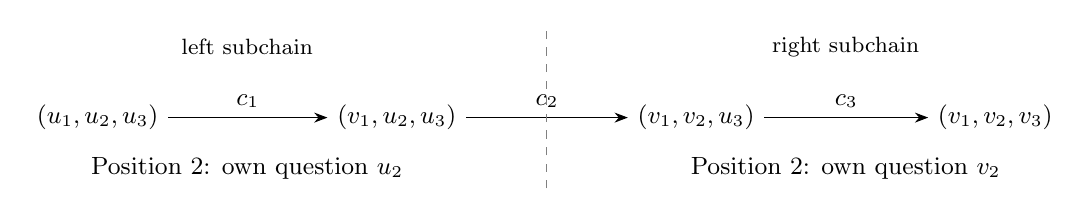
\begin{tikzpicture}[>=Stealth, every node/.style={font=\small}]
\node (a) at (0,0) {$(u_1,u_2,u_3)$};
\node (b) at (3.8,0) {$(v_1,u_2,u_3)$};
\node (c) at (7.6,0) {$(v_1,v_2,u_3)$};
\node (d) at (11.4,0) {$(v_1,v_2,v_3)$};
\draw[->] (a) -- node[above] {$c_1$} (b);
\draw[->] (b) -- node[above] {$c_2$} (c);
\draw[->] (c) -- node[above] {$c_3$} (d);
\draw[dashed,gray] (5.7,-0.9) -- (5.7,1.1);
\node at (1.9,-0.65) {Position $2$: own question $u_2$};
\node at (9.5,-0.65) {Position $2$: own question $v_2$};
\node[font=\footnotesize] at (1.9,0.9) {left subchain};
\node[font=\footnotesize] at (9.5,0.9) {right subchain};
\end{tikzpicture}
\caption{Four layers with the separating test $c_2$ left unconditioned.
Once $c_1,c_3$ are fixed, the left and right subchain data depend only
on the respective own question of $c_2$. Answer maps act in the position
indicated by each test.}
\label{fig:locality}
\end{figure}

Form a list of candidate left answers by taking position $h$
of every label in every $S_I^j$ for $j\in I$.
This gives at most $d$ elements of $\Sigma_L$, as a function of $u_h$
and fixed background. The analogous list for $J$ gives at most $d$
elements of $\Sigma_R$ as a function of $v_h$.
Choose deterministic orderings and pad each list to length $d$
with an arbitrary answer, also when the list is empty.

If $A_I$ and $A_J$ intersect, some left and right selected labels have
the same image at layer $r$. Equality in position $h$ says that
$\pi_{c_h}$ sends the associated left candidate to the right candidate:
on the left, exactly the test $c_h$ acts in that position, and on the
right the position is already a right-answer coordinate.
For each pair of list positions, selecting those answers for each
own question is a deterministic strategy for the original Label Cover
instance. Its success probability over the uniform $c_h$ is at most
$\sigma$. A union bound over the $d^2$ position pairs proves the
conditional bound, and averaging over the background proves the lemma.
\end{proof}

The fixed functions may depend on the entire instance and on
$\mathcal A$. This causes no loss of locality: they are fixed before
the sampling experiment, so evaluating the family at a tuple reveals
only that tuple. In particular, if two occurrences have the same own
question but different opposite questions or projections, the list
rule at that side uses identical data.

We have obtained bounded lists in a common answer set, and source
soundness controls intersections of lists on separated layer sets.
The next section turns this separation into a stronger property:
each listed answer can be assigned to one layer common to all of its
occurrences inside the sampled set $B$.

\section{Aligning the lists on a sampled set of layers}
\label{sec:alignment}

The terminal lists $A_I\subseteq M_r$ all have size at most $d$.
For the analytic argument, we need more than disjointness on separated
sets: each label should have a layer common to every set on whose list
it appears. These properties differ even for one label. A label that
occurs on the three sets $\{1,2\}$, $\{1,3\}$, and $\{2,3\}$ has no
common index, although none of these sets is separated from another.

The following abstract lemma supplies the common-index property on a
sampled $s$-element set. Its essential quantifier is that the sampling
law is chosen before the lists, with no dependence on the label universe.
This is what allows the same graph construction to handle every
independent set.

\begin{samepage}
\begin{lemma}[Distributional alignment]
For every pair of integers $s,d\geq 1$ and every real $\eta>0$, there exist
an integer $r\geq s$ and a rational probability distribution $\mu$ on
$\binom{[r]}s$ with the following property.\label{lem:alignment}
Let $M_*$ be any set, and let
$A_I\subseteq M_*$, $|A_I|\leq d$, be specified for every nonempty
$I\subseteq[r]$ with $|I|\leq s$. Assume that
\begin{equation}\label{align:separation}
 A_I\cap A_J=\varnothing
 \qquad\text{whenever }\max I<\min J.
\end{equation}
Then, with probability at least $1-\eta$ over $B\sim\mu$, there exists a map
$a:M_*\to B$ such that
\begin{equation}\label{align:conclusion}
 a(A_I)\subseteq I
 \qquad\text{for every nonempty }I\subseteq B.
\end{equation}
The map $a$ may depend on the list family and on $B$.
\end{lemma}
\end{samepage}

The complete proof is in Section~\ref{sec:alignment-proof}.
It replaces labels by their finite equality patterns, applies minimax
and Ramsey homogenization, and obtains an order-invariant random
pattern. In that limit, separated disjointness forces every label to
have an index common to all of its occurrences. We now apply the
lemma to the lists already extracted from an independent set.

Fix $\eps>0$, and suppose that the layer count $r$ and law $\mu$ in
the graph construction are supplied by Lemma~\ref{lem:alignment}
for $s,d,\eta=\eps$. Section~\ref{sec:parameters} will choose these
data after the alphabet-independent bound $d$ is fixed and before
choosing the Label Cover instance.

\begin{definition}
A pair consisting of a chain and a set $B\in\binom{[r]}s$ is
\emph{aligned} if there is a map $a:M_r\to B$ such that
$a(A_I)\subseteq I$ for every nonempty $I\subseteq B$.
\end{definition}

\begin{lemma}[Aligned pairs occur with high probability]
\label{lem:good-pairs}
Under these choices, for independent uniform chain sampling and
$B\sim\mu$, the probability that the pair is not aligned is at most
$4^r d^2\sigma+\eps$.
\end{lemma}

\begin{proof}
There are at most $4^r$ ordered pairs of subsets of $[r]$.
By Lemma~\ref{lem:separated-lists} and a union bound, the probability
that some separated pair of terminal lists intersects is at most
$4^r d^2\sigma$.
For each chain with no such intersection, Lemma~\ref{lem:alignment}
gives an alignment except for a set of $B$ of $\mu$-probability
at most $\eps$. Adding the two failure probabilities proves the bound.
\end{proof}

The lists were selected before $B$, and include the juntas for every
coefficient choice. An alignment for a fixed aligned pair can therefore
be chosen before the actual coefficient and rotation draws.
The next section uses this fixed alignment to control dependence on
one auxiliary phase for each layer in $B$.

\section{The coefficient test and soundness}
\label{sec:coefficient}

The remaining task is to bound the density of an independent set after
fixing an aligned pair of a chain and a selected set of layers.  We add
one auxiliary phase for each selected layer.  Alignment makes the
influence of a zero-coefficient layer small, whereas the geometric
coefficient distribution makes large influences at positive coefficients
unlikely.

Keep the tolerance $\eps>0$ of Section~\ref{sec:alignment}, and take
$\beta>0$ and $K\ge1$ from
Lemma~\ref{lem:influences} with $L=64$ and this $\eps$.
For the graph parameters of Section~\ref{sec:construction} and the
list-approximation tolerance $\gamma$ of Section~\ref{sec:lists}, assume
\begin{equation}\label{eq:parameter-bounds}
 \begin{gathered}
 L/m<\beta/2,\qquad \lambda K<\eps,
 \qquad (1-p_m)^s<\eps,\\
 \frac{s(2\gamma)^2}{\beta^2}<\eps,\qquad
 \frac{2L}{D}<\gamma,\qquad \frac{2Ls}{P}<\eps.
 \end{gathered}
\end{equation}
Section~\ref{sec:parameters} will choose constants satisfying these
inequalities. A coefficient equal to $1$ is called a \emph{full
coefficient}. Although its individual probability $p_m$ may be small,
the third inequality makes at least one of the $s$ coefficients full
with probability greater than $1-\eps$.

\begin{proposition}\label{prop:aligned-bound}
Assume \eqref{eq:parameter-bounds}. Suppose that the construction does not
take the clique branch, and let
$\mathcal A$ be a nonempty independent set of its output graph.  Form the
functions and lists associated with $\mathcal A$ as above.  For every
chain and $s$-element set $B$ admitting a map
\[
 a:M_r\longrightarrow B,
 \qquad a(A_I)\subseteq I
 \quad\text{for every nonempty }I\subseteq B,
\]
the conditional probability that the sampled output vertex belongs to
$\mathcal A$ is at most $6\eps$.
\end{proposition}

\begin{proof}
Fix such a chain, $B$, and a map $a$, before drawing any coefficients or
rotations.  Write $b=\min B$.
Since $f=1$ at every location of $\mathcal A$, it suffices to bound the
expected square of $F_b$ at the sampled grid location by $6\eps$.
We establish this through a continuous rotation experiment with auxiliary
phases.  Initially replace the discrete rotations
by independent uniform real variables
\[
 \theta_{j,\ell}\in[0,1),
 \qquad j\in B,\quad \ell\in M_j.
\]
All these variables are independent of the coefficient vector
$t\in\mathcal T_m^B$.  Introduce additional independent Haar-uniform
variables $z=(z_i)_{i\in B}\in\T^B$, and define
\begin{equation}\label{coeff:H}
 H(t,\theta;z)
 =F_b\left(\left(
 z_{a(\pi_{br}(\kappa))}
 +\sum_{j\in B}t_j\theta_{j,\pi_{bj}(\kappa)}
 \pmod 1\right)_{\kappa\in M_b}\right).
\end{equation}
For fixed $t,\theta$, the map from $z$ to the phase vector in
\eqref{coeff:H} is nonexpanding for the sup circle metrics: each output
coordinate uses just one coordinate of $z$.  Consequently $H$ is
$L$-Lipschitz as a function of $z$, independently of $s$ and of all label
cardinalities.  It is bounded by one in absolute value.  A simultaneous
half-shift of the $z$ coordinates half-shifts every input coordinate of
$F_b$, so oddness gives
\begin{equation}\label{coeff:mean-zero}
 \E_z H(t,\theta;z)=0.
\end{equation}

Let $E_i$ average only $z_i$ and let $Q_i=\id-E_i$, an orthogonal
projection of norm one.  We use the notation
\[
 D_i(t,\theta)=\|Q_iH(t,\theta;\cdot)\|_{L^2(\T^B)},
 \qquad X(t,\theta)=\E_z H(t,\theta;z)^2.
\]
By Lemma~\ref{lem:influences} and \eqref{coeff:mean-zero},
\begin{align}
 X(t,\theta)>\eps
 &\quad\Longrightarrow\quad
 \max_{i\in B}D_i(t,\theta)\ge\beta,
 \label{coeff:variance-detection}\\
 \#\{i\in B:D_i(t,\theta)\ge\beta/2\}
 &\le K
 \quad\text{for every }t,\theta.
 \label{coeff:count}
\end{align}

\paragraph{Zero coefficients.}
Let
\[
 \mathcal F=\{t:\text{some }t_j=1\}
\]
be the event that a full coefficient is present.  Fix $t\in\mathcal F$
and an index $i\in B$ with $t_i=0$.  Choose $j\in B$ with $t_j=1$;
necessarily $j\ne i$.  Put $I=B\setminus\{i\}$ and $c=\min I$.
The set $I$ is nonempty.  In the subchain function
$h_{I,t|_I}$ from \eqref{eq:subchain-functions}, leave all rotation
blocks unchanged except block $j$, where we substitute
\begin{equation}\label{coeff:shift}
 \theta'_{j,\ell}
 =\theta_{j,\ell}+z_{a(\pi_{jr}(\ell))}\pmod 1,
 \qquad \ell\in M_j.
\end{equation}
Here and below a phase used as a real rotation is represented in
$[0,1)$.  For each fixed $z$, this substitution preserves the product
uniform distribution of the rotation inputs.  Even when several
coordinates receive the same shift, each coordinate undergoes a fixed
translation, so their conditional joint law remains the same product
law.

To compare the two function evaluations, let $y\in\T^{M_c}$ be the
phase vector in $h_{I,t|_I}(\theta')$.  For every $\kappa\in M_b$,
composition of the projections gives
\begin{equation}\label{coeff:pullback-identity}
 y_{\pi_{bc}(\kappa)}
 =z_{a(\pi_{br}(\kappa))}
   +\sum_{k\in B}t_k\theta_{k,\pi_{bk}(\kappa)}
   \pmod 1.
\end{equation}
Indeed, the omitted $i$ term is zero, and the changed $j$ term has
coefficient exactly one.  This last fact is essential: reducing the
shifted rotation modulo one before multiplying would not in general be
valid at a fractional coefficient.  Thus
$H(t,\theta;z)=F_b(y\circ\pi_{bc})$.  If $c=b$ the two evaluations
are identical; if deleting $i$ changes the minimum layer, the
compatibility bound \eqref{eq:compatibility} still gives
\begin{equation}\label{coeff:deletion-error}
 |H(t,\theta;z)-h_{I,t|_I}(\theta')|
 \le 2L/D<\gamma.
\end{equation}

Let $g_{I,t|_I}$ be the fixed junta approximating $h_{I,t|_I}$ in
$L^2$ norm to error less than $\gamma$.  Its selected coordinates in
block $k$ belong to $S_I^k$.  Product-law preservation for every fixed
$z$ implies
\[
 \big\|h_{I,t|_I}(\theta')-g_{I,t|_I}(\theta')\big\|_{L^2(\theta,z)}
 <\gamma.
\]
Moreover, the composed function $g_{I,t|_I}(\theta')$ is pointwise
independent of $z_i$.  Only the modified block $j$ introduces any $z$
dependence.  Every selected coordinate $\ell\in S_I^j$ satisfies
$\pi_{jr}(\ell)\in A_I$ by \eqref{eq:terminal-lists}, and alignment
therefore gives $a(\pi_{jr}(\ell))\in I$.  Combining this observation
with \eqref{coeff:deletion-error} and applying the contraction $Q_i$
on the full product space yields
\begin{equation}\label{coeff:zero-bound}
 \E_\theta D_i(t,\theta)^2
 =\|Q_iH\|_{L^2(\theta,z)}^2
 \le
 \big\|H-g_{I,t|_I}(\theta')\big\|_{L^2(\theta,z)}^2
 <(2\gamma)^2.
\end{equation}
This estimate holds for every fixed $t\in\mathcal F$ with $t_i=0$.
Markov's inequality, followed by a union bound over the $s$ indices,
therefore gives
\begin{equation}\label{coeff:zero-probability}
 \Pr_{t,\theta}\bigl(
 t\in\mathcal F,\ 
 \exists i\in B:\ t_i=0,\ D_i(t,\theta)\ge\beta
 \bigr)
 \le \frac{s(2\gamma)^2}{\beta^2}<\eps.
\end{equation}

\paragraph{Positive coefficients.}
We next bound large influences at positive coefficient levels.  This
step does not assume that a full coefficient is present.  Fix $i$,
all rotations $\theta$, and all coefficients other than $t_i$.
For $0\le k\le m$, let $H_k$ denote \eqref{coeff:H} with $t_i=k/m$,
and put $d_k=\|Q_iH_k\|_2$.  Changing one coefficient by $1/m$
changes each phase coordinate by circle distance at most $1/m$, since
the rotations lie in $[0,1)$.  The norm-one property of $Q_i$ gives
\begin{equation}\label{coeff:one-step}
 |d_k-d_{k-1}|
 \le\|Q_i(H_k-H_{k-1})\|_2
 \le L/m<\beta/2
 \qquad(1\le k\le m).
\end{equation}
Write $p_k=\lambda^k/\sum_{h=0}^m\lambda^h$ for the probability
of coefficient level $k/m$.  Since $p_k=\lambda p_{k-1}$,
\eqref{coeff:one-step} implies, for the fixed background data,
\begin{align*}
 \sum_{k=1}^m p_k\mathbf 1_{\{d_k\ge\beta\}}
 &\le\lambda\sum_{h=0}^{m-1}
              p_h\mathbf 1_{\{d_h\ge\beta/2\}}\\
 &\le\lambda\sum_{h=0}^m
              p_h\mathbf 1_{\{d_h\ge\beta/2\}}.
\end{align*}
Integrating over the fixed data and summing over $i\in B$, we obtain
from \eqref{coeff:count}
\begin{equation}\label{coeff:positive-probability}
 \begin{split}
 \Pr_{t,\theta}\bigl(
 \exists i\in B:\ t_i>0,\ D_i(t,\theta)\ge\beta
 \bigr)
 &\le\lambda\sum_{i\in B}
          \Pr_{t,\theta}(D_i(t,\theta)\ge\beta/2)\\
 &\le\lambda K<\eps.
 \end{split}
\end{equation}
Decreasing a level can destroy the only full coefficient.  This causes
no restriction here: \eqref{coeff:count} holds for every coefficient
vector, including all images of the one-level decrease.

\paragraph{From influences to mean square.}
The parameter choices in \eqref{eq:parameter-bounds} give
$\Pr(t\notin\mathcal F)<\eps$.  By
\eqref{coeff:variance-detection}, the event $X(t,\theta)>\eps$ is
contained in the union of this event and the two events bounded in
\eqref{coeff:zero-probability} and
\eqref{coeff:positive-probability}.  Consequently
\[
 \Pr_{t,\theta}(X(t,\theta)>\eps)<3\eps.
\]
Since $0\le X\le1$, it follows that
\begin{equation}\label{coeff:mean-square}
 \E_{t,\theta,z}H(t,\theta;z)^2
 =\E_{t,\theta}X(t,\theta)
 \le\eps+\Pr(X>\eps)<4\eps.
\end{equation}
We now remove the auxiliary phases and return to the actual grid
sampling.  This is the only remaining passage from the analytic test
to the conditional vertex density.

\paragraph{Removing the phases and discretizing.}
Define the continuous location
\[
 x(t,\theta)
 =\left(\sum_{j\in B}t_j\theta_{j,\pi_{bj}(\kappa)}
          \pmod 1\right)_{\kappa\in M_b}.
\]
For every fixed $t\in\mathcal F$, choose an index $j$ with $t_j=1$.
Applying the translation \eqref{coeff:shift} to this block absorbs
every $z$ term in \eqref{coeff:H}.  For each fixed $z$ the translated
rotation array again has exactly its original product law.  Hence
\begin{equation}\label{coeff:absorption}
 \E_{\theta,z}H(t,\theta;z)^2
 =\E_\theta F_b(x(t,\theta))^2
 \qquad(t\in\mathcal F).
\end{equation}
The choice of the full block may depend on $t$, because this equality
is asserted separately for every fixed coefficient vector.  In
particular, \eqref{coeff:mean-square} implies
\begin{equation}\label{coeff:continuous-bound}
 \E_{t,\theta}\!\left[
 \mathbf 1_{\mathcal F}(t)F_b(x(t,\theta))^2\right]<4\eps.
\end{equation}

Couple the discrete rotations to the continuous ones by
\[
 \widehat\theta_{j,\ell}
 =\frac{\lfloor P\theta_{j,\ell}\rfloor}{P}.
\]
They have the required independent uniform grid law.  Each input
coordinate changes by less than $1/P$, so the sup circle distance
between $x(t,\theta)$ and $x(t,\widehat\theta)$ is at most $s/P$.
The Lipschitz bound and the range $[-1,1]$ therefore imply
\begin{equation}\label{coeff:grid-error}
 \left|F_b(x(t,\theta))^2
       -F_b(x(t,\widehat\theta))^2\right|
 \le 2Ls/P<\eps.
\end{equation}
Combining \eqref{coeff:continuous-bound},
\eqref{coeff:grid-error}, and $\Pr(t\notin\mathcal F)<\eps$ gives
\begin{equation}\label{coeff:discrete-bound}
 \E_{t,\widehat\theta}
       F_b(x(t,\widehat\theta))^2
 <4\eps+\eps+\eps=6\eps.
\end{equation}
The discrete location belongs to the grid of denominator $D=mP$, so
$F_b$ equals the original grid function $f$ there.  That function
equals one at every location of a vertex of $\mathcal A$.
Thus the indicator that the sampled vertex belongs to $\mathcal A$
is pointwise bounded by $F_b(x(t,\widehat\theta))^2$.
This remains true when several distinct vertices have the same
location.  Inequality~\eqref{coeff:discrete-bound} proves the
proposition.
\end{proof}

\section{Choosing the constants and completing the reduction}
\label{sec:parameters}

The construction and its analysis have identified all the required
properties of the fixed parameters. We now choose them in an order
that makes the graph reduction possible. The key point is that the
list bound $d$ is fixed before the layer count and the source soundness,
so it cannot depend on the Label Cover alphabets.

Fix a rational $0<\delta<1/3$ and a rational
$0<\eps<\delta/8$. Set $L=64$ and take $\beta,K$ from
Lemma~\ref{lem:influences} for $L,\eps$.
Choose a positive integer $m$ with $L/m<\beta/2$, then a rational
$0<\lambda<1$ with $\lambda K<\eps$.
The coefficient law \eqref{eq:coefficient-law} is now fixed.
Since its probability $p_m$ of a full coefficient is positive, choose
an integer $s\ge2$ with $(1-p_m)^s<\eps$.

Next choose $\gamma>0$ sufficiently small that
$s(2\gamma)^2/\beta^2<\eps$, and then choose an even positive integer
$P$ sufficiently large that, with $D=mP$,
\[
 \frac{2L}{D}<\gamma,
 \qquad \frac{2Ls}{P}<\eps.
\]
This establishes every inequality in \eqref{eq:parameter-bounds}.
Lemma~\ref{lem:subchain-lists} gives the alphabet-independent bound
\[
 d=\max\{1,J(sL,\gamma)(m+1)^s\}.
\]
Apply Lemma~\ref{lem:alignment} to $s,d,\eta=\eps$, obtaining
$r\ge s$ and a rational law $\mu$ on $\binom{[r]}s$.
Finally choose a rational $\sigma\in(0,1)$ with
\begin{equation}\label{eq:source-soundness}
 4^r d^2\sigma<\eps.
\end{equation}
Only now invoke Theorem~\ref{thm:label-cover} for this fixed $\sigma$.
Its constant alphabets may be large, but no preceding choice depends
on their sizes or on the input formula.

All objects used to run the reduction are finite integers or finite
rational probability tables. For each fixed $\delta$, choose them
once and incorporate their finite descriptions into one algorithm.
Neither a uniform runtime as $\delta\to0$ nor an algorithm computing
all constants from $\delta$ is asserted or needed. There is no
input-dependent advice. The real tolerances, continuous functions,
junta approximants, and alignments enter only the analysis.

\begin{proof}[Proof of Theorem~\ref{thm:main}]
It suffices to treat rational $0<\delta<1/3$: for a fixed real
threshold, choose a fixed rational $0<\delta_0<\delta$ and use the
reduction for $\delta_0$.
Fix rational $\delta$ and choose the constants as above, with
$8\eps<\delta$. Use the preprocessing and graph construction of
Section~\ref{sec:construction}.

The two preprocessing branches already have the required promises.
A formula with no remaining clauses is satisfiable and produces a
one-vertex graph. An empty clause certifies unsatisfiability and
produces $K_q$, where $q>1/\delta$ and hence $1/q<\delta$.
For every other input, Proposition~\ref{prop:encoding} gives a
deterministic polynomial-time construction of a nonempty finite simple
unweighted graph. If the formula is satisfiable, its Label Cover
instance has value one, and Lemma~\ref{lem:completeness} supplies a
proper three-coloring of every output vertex.

Suppose instead that the formula is unsatisfiable, so its Label Cover
value is at most $\sigma$. If the metric clique branch occurs, the
output again has independent-set density $1/q<\delta$.
Otherwise, let $\mathcal A$ be any nonempty independent set of the
output graph. Lemma~\ref{lem:good-pairs} and
\eqref{eq:source-soundness} bound the probability of an unaligned
chain--$B$ pair by $2\eps$.
At every aligned pair, Proposition~\ref{prop:aligned-bound} bounds
the conditional probability of sampling $\mathcal A$ by $6\eps$;
at other pairs it is at most one. The multiplicity expansion in
Proposition~\ref{prop:encoding} makes this sampling law exactly the
uniform law on output vertices. Hence
\[
 \frac{|\mathcal A|}{|V(G)|}
 \le 6\eps+2\eps
 =8\eps<\delta.
\]
The empty independent set satisfies the same strict bound because
the graph is nonempty. Maximizing over all independent sets proves
the required soundness promise.
\end{proof}

\section{Proof of distributional alignment}
\label{sec:alignment-proof}

We prove Lemma~\ref{lem:alignment}, the combinatorial input used to
choose the sampling law on layer sets. The argument depends only on
the list bound and the order of the indices; it has no graph-theoretic
or analytic hypotheses.

\begin{proof}[Proof of Lemma~\ref{lem:alignment}]
Call $B$ \emph{bad} if no map in \eqref{align:conclusion} exists.  For each
label $x$ that appears on a list indexed inside $B$, consider
\[
 \bigcap\{I:\varnothing\ne I\subseteq B,\ x\in A_I\}.
\]
The set $B$ is bad exactly when one of these intersections is empty.
Indeed, a nonempty intersection permits a choice of $a(x)$ independently
for each appearing label; labels absent from all these lists may be sent to
any element of the nonempty set $B$.

We first prove that for every $\xi>0$, some $r\geq s$ admits a real
probability distribution on $\binom{[r]}s$ under which every list family
satisfying \eqref{align:separation} has bad-set probability at most $\xi$.
The proof has three steps.  Finite minimax turns a failure of this assertion
into random list patterns making every $s$-set bad with positive
probability.  Ramsey homogenization produces an order-invariant limiting
pattern on the rationals.  Finally, an invariant-cut argument shows that
such a limiting pattern has no bad sets.

\paragraph{Finite patterns and minimax.}
Order each list arbitrarily.  On a finite ordered index set, retain only
the length of each list and the equality relation among its occupied
slots.  Each list has at most $d$ slots, and no two occupied slots of one
list are equal.  There are finitely many resulting patterns.  Every actual
list family gives such a pattern, and conversely a pattern is realized by
using its equivalence classes as labels.  Thus the original label universe
has no further role in either separation or badness.

Write $\mathcal C_r$ for the finite set of patterns on $[r]$ satisfying
\eqref{align:separation}, and put
\[
 b(B,C)=\boldsymbol{1}\{B\text{ is bad in }C\},
 \qquad B\in\binom{[r]}s,\ C\in\mathcal C_r.
\]
If the assertion with tolerance $\xi$ were false for every $r$, then for
each $r\geq s$ the finite minimax theorem \cite{vonNeumann1928} would give
\[
 \min_{\nu}\max_{C\in\mathcal C_r}
       \E_{B\sim\nu}b(B,C)
 =
 \max_{\rho}\min_{B\in\binom{[r]}s}
       \E_{C\sim\rho}b(B,C)
 >\xi.
\]
Here $\nu$ and $\rho$ range over the two finite probability simplices;
their compactness ensures that the extrema are attained.  Consequently,
for every $r\geq s$ there would be a random allowed pattern $C_r$ such that
\begin{equation}\label{align:uniform-bad}
 \Pr(B\text{ is bad in }C_r)\geq\xi
 \qquad\text{for every }B\in\binom{[r]}s.
\end{equation}
Assume this counterstatement for the remainder of the argument.

\paragraph{An order-invariant limit.}
The homogenization step applies finite Ramsey theory \cite{Ramsey1930}
to discretized probability patterns, following the kind of extraction
used by Trotter and Winkler \cite{TrotterWinkler1998}. We give the
particular argument needed here in full.
For $t\geq1$, let $\mathcal P_t$ denote the finite set of all allowed
patterns on $[t]$, using lists on subsets of size at most $s$.
Restriction to an ordered subset, followed by its increasing identification
with an initial interval of integers, defines a map between the appropriate
pattern spaces.

Fix $k\geq s$.  For each $1\leq t\leq k$ and each $t$-subset $J$ of
$[r]$, the restriction of $C_r$ to $J$ has a probability vector in the
finite simplex on $\mathcal P_t$.  Color $J$ by this vector with every
entry placed in a bin of width at most $1/k$.  The number of colors depends
only on $s,d,t,k$, not on $r$.  Successive applications of the finite
Ramsey theorem, with the required intermediate set sizes chosen backwards,
give the following when $r$ is sufficiently large: there is a $k$-element
set $H_k$ on which all the colorings, for $1\leq t\leq k$, are
homogeneous.  Passing to a subset preserves each homogeneity already
obtained.  In particular, the induced pattern laws on any two $t$-subsets
of $H_k$ differ by at most $1/k$ in every coordinate.

Let $P_t^{(k)}$ be the law on the first $t$ points of $H_k$.  If
$t\leq u\leq k$ and $J\in\binom{[u]}t$, restricting $P_u^{(k)}$ to
$J$ gives the law on the corresponding $t$-subset of $H_k$.  Therefore
\begin{equation}\label{align:approx-consistency}
 \left|
   \bigl(P_u^{(k)}|_J\bigr)(C)-P_t^{(k)}(C)
 \right|\leq\frac1k
 \qquad(C\in\mathcal P_t).
\end{equation}
Compactness of each finite simplex and a diagonal subsequence as
$k\to\infty$ produce limiting laws $P_t$ for every $t$.  Taking limits
in \eqref{align:approx-consistency} gives exact consistency under every
ordered restriction:
\begin{equation}\label{align:consistency}
 P_u|_J=P_t
 \qquad(t\leq u,\ J\in\binom{[u]}t).
\end{equation}
Moreover, \eqref{align:uniform-bad} gives
\begin{equation}\label{align:limit-bad}
 P_s(\text{the full index set is bad})\geq\xi.
\end{equation}

Assign the law $P_t$ to every increasing $t$-tuple of rational indices.
The consistency in \eqref{align:consistency} constructs a countable random
array of list lengths and equality relations indexed by the nonempty
$I\subseteq\Q$ of size at most $s$.  For completeness, enumerate $\Q$
and successively extend the pattern on the first $n$ enumerated indices
to the first $n+1$, using the conditional probabilities supplied by their
consistent finite laws.  The choices on zero-probability conditioning
events are immaterial.  Every finite set of rational indices then has its
specified law.

All equivalence-relation axioms, distinctness within a list, and separated
disjointness hold simultaneously almost surely: each violation involves
finitely many indices, and there are only countably many possible
violations.  The array's law is invariant under every increasing
automorphism of $\Q$, because its finite laws depend only on order.
Equation~\eqref{align:limit-bad} says that every fixed rational $s$-set
still has bad probability at least $\xi$.

We have thus retained the positive bad-set probability while removing all
distinctions between index sets having the same order type.  We next show
that this order invariance, together with separated disjointness, forces
every label to have an index common to all its occurrences.

\paragraph{An invariant cut for each label.}
Fix a nonempty $I\subseteq\Q$, $|I|\leq s$, and one of its $d$ possible
slots.  Let $E$ be the event that this slot is occupied.  On $E$, write
$\mathcal L$ for its equivalence class of occupied slots, and define
\begin{equation}\label{align:cut}
 p=\sup\{\min J:\text{a slot at }J\text{ belongs to }\mathcal L\}.
\end{equation}
The set whose supremum is taken contains $\min I$.  It is bounded above
by $\max I$, since an occurrence at $J$ with $\min J>\max I$ would
violate separated disjointness.  Thus
\begin{equation}\label{align:cut-hull}
 \min I\leq p\leq\max I
 \qquad\text{on }E.
\end{equation}
The random variable $p$ is measurable on $E$: the occurrence family is
countable, and testing whether its supremum is at most a given real number
is a countable intersection of measurable conditions on slots.

Every increasing automorphism $g$ of $\Q$ extends uniquely to an increasing
homeomorphism $\bar g$ of $\R$.  Transporting the array by $g$ transports
the occurrence family in \eqref{align:cut} and sends its supremum to
$\bar g(p)$.  If $g$ fixes $I$ pointwise, it also fixes the selected slot
and its occupancy event.  Hence the finite measure
\[
 \nu(U)=\Pr(E\text{ and }p\in U),
 \qquad U\subseteq\R\text{ Borel},
\]
is invariant under all such $\bar g$.  This formulation also covers
$\Pr(E)=0$ without conditioning on a null event.

Let $a<b$ be consecutive points of $I$.  For any rational
$a<q<q'<b$, there is an increasing automorphism of $\Q$ fixing $I$
pointwise and carrying $q$ to $q'$.  For example, use a piecewise linear
increasing bijection of $\R$ that is the identity off $[a,b]$, maps $q$
to $q'$, and is linear on $[a,q]$ and $[q,b]$.  Its rational breakpoints
and rational slopes make it a bijection of $\Q$.  Invariance gives
\[
 \nu(({-\infty},q])=\nu(({-\infty},q']),
 \qquad\text{so}\qquad \nu((q,q'])=0.
\]
Countably many such rational intervals cover $(a,b)$, whence
$\nu((a,b))=0$.  Together with \eqref{align:cut-hull}, this proves
\begin{equation}\label{align:cut-index}
 \Pr(E\text{ and }p\notin I)=0.
\end{equation}
If $I$ is a singleton, \eqref{align:cut-index} follows directly from
\eqref{align:cut-hull}.

There are only countably many possible slots, so
\eqref{align:cut-index} holds simultaneously at every occupied slot with
probability one.  Equivalent slots have exactly the same occurrence
family and hence the same supremum $p$.  It follows that every equivalence
class has a common index in all the sets on whose lists it occurs.
In particular, on every finite rational $s$-set $B$, every label appearing
inside $B$ has a nonempty intersection of its occurrence sets there.
Thus no such $B$ is bad, contradicting \eqref{align:limit-bad} and
$\xi>0$.  This proves the assertion with real probabilities.

\paragraph{Rational probabilities.}
Choose $0<\xi<\eta$ and obtain $r$ and a real distribution $\mu_0$ with
bad-set probability at most $\xi$ for every allowed pattern.  Approximate
$\mu_0$ by a rational point $\mu$ of the same finite simplex with
\[
 \sum_{B\in\binom{[r]}s}|\mu(B)-\mu_0(B)|<\eta-\xi.
\]
Every bad-set indicator takes values in $[0,1]$, so this changes its
expectation by less than $\eta-\xi$, uniformly over all patterns.
The distribution $\mu$ therefore has the required guarantee.
\end{proof}

\begin{remark}\label{align:effective}
For rational $\eta>0$, the finite data in Lemma~\ref{lem:alignment} can
also be found by a terminating search.  Enumerate $r\geq s$, enumerate
its finitely many allowed slot patterns, and minimize their maximum
bad-set probability by a rational linear program.  Search until its
optimum is less than $\eta$.  The proof with a smaller tolerance guarantees
termination.  No bound on the label universe, or oracle describing it, is
needed.
\end{remark}

\bibliographystyle{plain}
\bibliography{references}
\end{document}
